\section{Device fabrication}
\label{sec:fabrication}

The following recipes and procedures are based on extensive prior work of the group of Dr.~Srijit Goswami at QuTech, TU Delft, and were further developed in close collaboration with Dr.~Nikos Papadopoulos.

\subsection{The art of making encapsulated graphene devices}

Fabrication of graphene Josephson junctions is a tedious process:
% 
In contrast to integrated circuits, where the active materials are homogeneously deposited over an entire substrate, the best graphene devices to date are not fabricated using scalable techniques, but rather each device is manually assembled and crafted, thus requiring significant efforts, since no two devices have the same exact shape.

Wafer-scale graphene fabrication is usually achieved by chemical vapour deposition of single layer graphene on copper foils.
% 
However, only until recently did the thus deposited films exhibit sufficiently low defect densities, which would otherwise result in inferior device quality.
% 
Transferring the graphene layer from its growth to the final substrate often contaminates both graphene and final substrate, which typically result in low device quality.
% 
Finally, even in the cases where transferred graphene results in low defect and residue densities, patterning into the final device shape always results in contaminations, most often due to organic resist residues.

Since graphene is really only a single atom thick and thus all electronic transport takes place at its surface, contaminations on either side will result in charge carrier scattering and degrade the device performance.
% 
Till this day, the devices with highest electronic quality, exhibiting phenomena such as ballistic transport, hydrodynamics, or superconductivity, rely on single layer graphene manually exfoliated from bulk graphite crystals~\cite{???,???,???}.


Additionally, it is often required to change the carrier density in the graphene layer, for which a gate electrode separated by a dielectric is needed.
% 
Because of the single-layer nature of graphene, it conforms very well to any surface roughness and is very sensitive to trapped charges in the dielectric layers, which called for an ideal gate dielectric.
% 
In 2010, Dean \textit{et al.}~\cite{dean_boron_2010} realized the use of hexagonal Boron Nitride (BN) as the (until now) best dielectric and capping layer for graphene devices, showing vast improvements with respect to device mobility.

Like graphene, BN has a hexagonal lattice, albeit consisting of two sub-lattices of boron and nitride atoms, and with a lattice mismatch of \SI{1}{\percent} to graphene.
% 
BN can be exfoliated from bulk crystals to thin insulating films of arbitrary layer number and signifcantly lower surface roughness than any other dielectric, making it a perfect match for graphene encapsulation.
% 
The highest quality BN crystals, i.e. the ones exhibiting the lowest charge defect density, are the ones made by ultra-high pressure ??? by Kenji Watanabe and Takashi Taniguchi at NIMS, Japan.

As confirmed by atomic force and scanning tunneling microscopy, SLG on BN exhibits a significantly lower roughness compared to samples on \ce{SiO2}, until then the standard dielectric for graphene devices.
% 
In addition, variations in the local density of states of SLG on BN can thus be reduced by a factor ten, while charge fluctuations are suppressed by a factor 100, as compared to SLG directly on \ce{SiO2}~\cite{xueScanningTunnellingMicroscopy2011,deckerLocalElectronicProperties2011}.
% 
Complete screening of any trapped charges in the dielectric layer can finally be achieved with gate electrodes out of graphite instead of conventional metals~\cite{ponomarenkoTunableMetalInsulator2011,ametNovelPhenomenaDriven2014}.

However, assembling a heterostructure of BN-G-BN, with subsequent patterning, and deposition of gate metals and dielectrics results in an extensive and long process, with processes varying between most research groups.
% 
In the following, we will detail the fabrication procedure used in the course of this thesis that resulted in the best measured devices.

\subsubsection{Substrate cleaning and flake exfoliation}

All BN-G-BN heterostructures are based on SLG and few-layer BN exfoliated from bulk highly oriented pyrolithic graphite (HOPG) and NIMS, respectively.
% 
Identifying flakes of suitable thickness is done by estimation the layer number and thickness from optical images.
% 
For optimal contrast, we used silicon substrates with \SI{285}{\nano\meter} of thermal \ce{SiO2}~\cite{blakeMakingGrapheneVisible2007}, diced into \SI{6x6}{\milli\meter} pieces from \SI{4}{inch} wafers from ???.
% 
Details on dicing parameters are given in Sec.~\ref{sec:fab-packaging}.

As mentioned earlier, any organic residues that come in contact with graphene will very likely lead to inferior device performance.
% 
Specifically, after dicing the chips, they need to be cleaned extensively in order to remove any leftovers from the dicing resist.
% 
To this end, diced chips are placed in a teflon holder and transferred through four \SI{50}{\milli\liter} glass beakers filled with acetone, acetone, isopropyl alcohol (isoporpanol, IPA) and IPA, each time ultrasonicated for \SI{5}{\minute}.
% 
The chips can either be blow-dried one by one using high-pressure nitrogen gas, or by rinsing the teflon holder with the chips still on it in three water baths and placing it on a petri dish in an oven.
% 
To remove acetone and IPA residues, the chips ultrasonicated for \SI{5}{\minute} in nitric acid and blow-dried after rinsing in water.
% 
We found that an additional soft oxygen plasma to functionalize the \ce{SiO2} surface (\SI{200}{sccm} of \ce{O2}, \SI{600}{\watt}, \SI{2}{\minute}, no cage inside the Tepla) just before, i.e. not more than \SI{15}{\minute} prior to, flake exfoliation increased flake exfoliation yield, regardless of graphene or BN.


Flake exfoliation is achieved by manually thinning down bulk crystals until micron-sized flakes of only one or two (SLG, BLG) or a few tens of layers (BN) thickness are left on a chip.
% 
The author estimates that there are as many different ways of flake exfoliation as there are researchers working on this procedure.
% 
The procedure that worked best for us concerning BN exfoliation consists of placing individual BN crystallites (approximately a few $(\SI{100}{\micro\meter})^3$ in volume) on a piece of \textit{Scotch} tape \textit{"Magic"} or \textit{Nitto} tape, and subsequently folding over said piece of tape numerous times, such that one acquires a closed layer of thin BN crystallites.
% 
In the case of graphene, we would peel off a preferably closed film of graphite from a single \SI{1x1}{\centi\meter} HOPG crystal with a piece of tape, followed by subsequent folding of the piece of tape until we acquired a homogeneous, yet closed film of thin graphite.

Once we were satisfied with the tape template, we would use pre-cut \SI{8x8}{\milli\meter} pieces of clean tape to peel off crystals from the template, the press the side with crystals on the small piece of tape onto a previously cleaned substrate, keep pressure applied using our index finger or thumb for approximately \SI{30}{\second}, then transfer the substrate with the tape still on to a hot plate and leave the substrate sit on the hot plate for \SIrange{2}{5}{\minute}.
% 
We found highest flake densities for temperatures of \SI{50}{\celsius} for \textit{Nitto} and \SI{100}{\celsius} for \textit{Magic} tape.
% 
Finally, the chip was transferred off the hot plate, left to cool for \SI{1}{\minute} and the tape would be gently peeled off, while holding the substrate in place with a pair of tweezers.
% 
During this process, no further pressure should be applied to the tape as this usually resulted in lots of tape residues on the chip.


The process of exfoliation turns out to be a tradeoff between getting as many flakes as possible, and getting the lowest tape residues possibles.
% 
\textit{Magic} tape has a higher adhesive strength, thus resulting in a higher flake density and predominantly large flakes (i.e. $>\SI{20x20}{\micro\meter}$) than \textit{Nitto} tape.
% 
On the other hand, this comes at the cost of more tape residues on both the substrate and the individual flakes.
% 
Tape residues can lead to enhanced charge carrier scattering of graphene films, thus severely limiting device quality.
% 
Additionally, they increase the chance of bubble formation (see below), thus limiting the available sample space.
% 
Tape residues can be entirely removed by thermal annealing at \SI{400}{\celsius} in  an \ce{Ar+H2} atmosphere.
% 
However, it extremely difficult to pick up or transfer flakes treated in this manner for heterostructure assembly (see below).
% 
While we found that annealing at temperatures below \SI{300}{\celsius} was still compatible with flake transfer, significantly less tape residues were removed this way.
% 
It is thus advisable to omit thermal annealing until the first lithography step.

\subsubsection{Heterostructure assembly}

%TODO: check for accuracy
Our transfer setup is the same as in Ref.~\cite{castellanos-gomezDeterministicTransferTwodimensional2014}, but upgraded with a heater stage capable of fast heating and cooling cycles between room temperature and \SI{150}{celsius}.
% 
We prepared the PPC solution by dissolving PPC at a \SI{15}{\percent} weight ratio in anisole at \SI{50}{\celsius}, while stirring with a fish magnet until everything was properly dissolved.
% 
Our assembly using PPC is based on Ref.~\cite{pizzoccheroHotPickupTechnique2016} with minor modifications adjusted to our transfer setup.
% 
For every pick-and-place step, we fixed the substrate from or to which to transfer the flakes with vacuum, and used a single glass slide with a bubble of PDMS covered with PPC.
%
Both glass slide and chip could be individually moved with micrometer screws.
%
The following steps describe our typical working process for achieving high-quality interfaces:

\begin{enumerate}
	\item Align the top BN flake with the center area of the PDMS/PPC template.
	%
	\item Lower the glass slide such that the PPC touches the substrate.
	%
	Take care that the PPC does not yet cover the flake, but touches down less than \SI{100}{\micro\meter} away from it.
	%
	\item Increase the stage temperature above \SI{55}{\celsius}.
	%
	The PDMS/PPC will expand and cover the flake, and adhesion between BN and PPC increase significantly.
	%
	\item Turn off the stage heater and wait for the stage to cool below \SI{40}{\celsius} (possibly with the help of a nitrogen gun).
	%
	At this stage, the adhesion between BN and PPC should exceed that of BN and substrate.
	%
	Now lifting the glass slide should rip the flake off the substrate.
	%
	If at this stage the intended flake did not get picked up, repeating the process by heating to \SIrange{80}{90}{\celsius} and then cooling down should result in a much higher yield, at cost of longer waiting times for the stage to cool down.
	%
	\item Place the chip with the graphene flake on the stage and align the flake with the BN on the glass slide below now.
	%
	Slowly lower the glass slide and set the stage temperature to \SI{110}{\celsius}. 
	%
	The hot air and deflected slide will make it difficult to align the two flakes, so extra care has to be taken at this step.
	%
	Once the stage has reached \SI{110}{\celsius}, bring stage and glass slide in contact as slowly as possible until the interface passes the Gr and BN, preferably letting the expanding PDMS do the work.
	%
	\label{assembly-start}
	%
	\item Increase the stage temperature to \SI{120}{\celsius} and then retract the glass slide, thus delaminating the top BN on the graphene flake.
	%
	\label{flake-delam}
	\item Anneal the Gr/hBN stack at \SI{170}{\celsius} for \SI{15}{\minute}.
	%
	\item Place PPC/PDMS glass slide above the chip, turn off the stage heater and bring the polymer in contact once the temperature is below \SIrange{70}{80}{\celsius}.
	% 
	\item Once the temperature drops below \SI{40}{\celsius}, retract the glass slide.
	%
	The Gr/hBn stack should get lifted off the substrate.
	%
	\label{assembly-stop}
	%
	\item For assembling the BN-G-BN sandwich, repeat steps \ref{assembly-start} - \ref{assembly-stop}.
	%
	If needed, transfer the sandwich to another substrate.
\end{enumerate}

Another polymer commonly used for heterostructure assembly is PC.
%
Its advantage over PPC is that it is a much stronger adhesive, so the intermediate flake delamination (step \ref{flake-delam}) can be skipped.
%
However, it needs to be kept in a fridge in order to not degrade, and cannot be spin-coated on the PDMS layer.
%
Instead, a droplet of PC is placed on a \SI{20x20}{\milli\meter} glass coverslip.
%
A second coverslip is dropped on the first one, thus spreading the droplet in between.
%
With care, but in a swift motion, we pull the top glass piece off, thus leaving behind a thin film of PC on the bottom glass slide, which can be peeled off using a piece of tape and placed on the PDMS stamp.
%
For flake transfer, we follow the above steps, except that the transfer takes place at a base temperature of \SI{110}{\celsius} instead of \SI{40}{\celsius}, and to activate the adhesion to PC, heating to \SIrange{130}{140}{\celsius} instead of \SIrange{80}{90}{\celsius} is required.


\begin{figure}
	\centering
	
\includegraphics[]{{chapter-experimental-methods/figs-fabrication/placeholder-large.svg}.png}
	\caption{
		\textbf{From bulk crystals to van der Waals heterostructures.}
		% 
		\textbf{A,} Bulk crystals of HOPG (grey) and hBN (white), together with a piece of wafer adhesive tape used to thin down these crystals by repeated folding and opening of the tape.
		% 
		The tape is pressed on a \SI{6x6}{\milli\meter} piece of silicon with \SI{285}{\nano\meter} \ce{SiO2} to enhance the optical contrast for monolayer graphene.
		% 
		\textbf{B,} Optical microscope image of a thin flake of graphite, exhibiting regions of single and multilayer graphene.
		% 
		\textbf{C,} Optical microscope image of an hBN flake of approximately \SI{30}{\nano\meter} thickness.
		% 
		All scalebars \SI{20}{\micro\meter}.
		% 
		\textbf{D,} Photograph of a glass slide with PDMS covered with a spun-on layer of PPC (approximately \SIrange{1}{2}{\micro\meter} thick).
		% 
		\textbf{E,} Typical sandwich assembly cycle for creating multi-layered van der Waals heterostructures:
		% 
		\textbf{i,} Polymer brought in contact with exfoliated flake on substrate at room temperature.
		% 
		\textbf{ii,} Heating substrate above glass transition temperature $T_g$ enhances the adhesion of the flake to the polymer significantly above the adhesion to the substrate.
		% 
		\textbf{iii,} Subsequent cooling of the substrate leads to stiffening of the polymer.
		% 
		Combined with rapid lifting of the glass slide, usually solely induced by the thermally shrinking polymer, lifts the flake off the substrate.
		% 
		By repeating steps \textbf{i}-\textbf{iii}, multiple flakes can be stacked on top of each other.
		% 
		\textbf{iv,} In order to deposit the finished heterostructure on a final substrate, the heterostructure is brought in contact with the substrate at room temperature, and the stage heated above the melting temperature of the polymer.
		% 
		Slow lifting of the glass slide leads to the structure remaining on the substrate, while the polymer can either remain fully stuck to the PDMS, or also remain on the substrate.
		% 
		\textbf{v,} Polymer residues can be removed in organic solvents such as anisole, NMP, PRS3000 or chloroform.
	}
	\label{fig:placeholder-large}
\end{figure}

\subsubsection{Challenges of heterostructure assembly}

We found that BN-G-BN stacks would often get washed away due to unsufficient adhesion to the sapphire substrate during processing.
Due to the low adhesion of BN to sapphire and silicon nitride, many stacks were washed off the final substrates during solving the polymer.
We did not observe this behaviour on silicon substrates, (cf. Fig.~\ref{fig:fab-hetero-challenge} (B) ), but had a yield of less than \SI{50}{\percent} on sapphire and \SI{0}{\percent} on silicon nitride films.

As in our paper, the polymer used for transfer (PC, PPC) has very strong adhesion to the metal areas of the shunts, ground planes and center conductors.
A long soak in NMP was able to remove the polymer at least visibly, but residual flakes had to be etched away in a separate step.

\begin{figure}
	\centering
	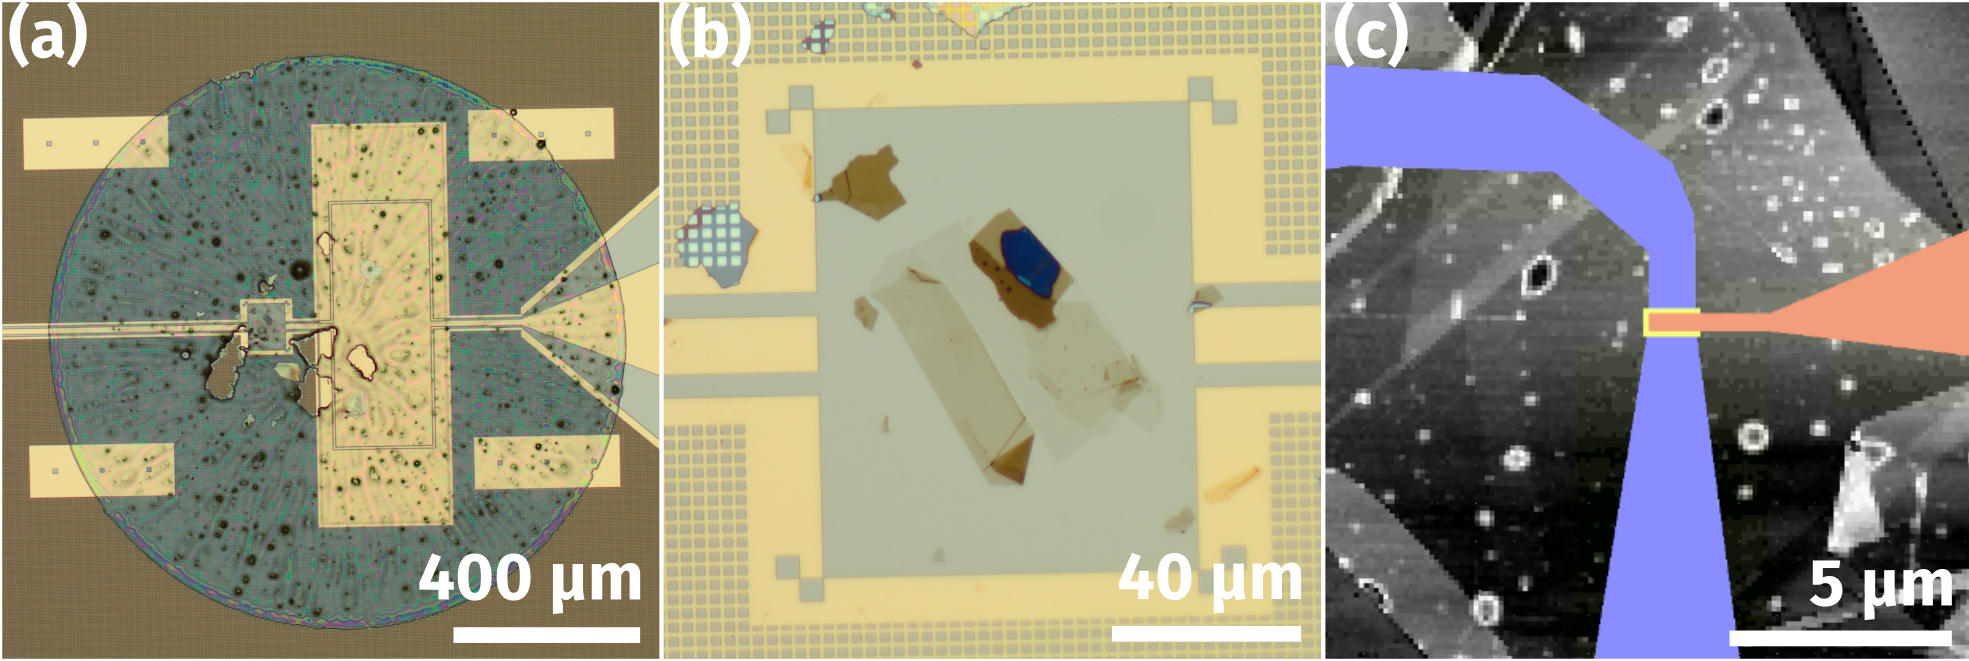
\includegraphics[]{{chapter-experimental-methods/figs-fabrication/fab-hetero-challenge.svg}.png}
	\caption{
		\textbf{Fabrication issues associated with van der Waals assembly.}
		% 
		\textbf{A,} Due to the good adhesion of the polymer to metal surfaces, after flake deposition the polymer would often get delaminated and the chip needs to be thoroughly cleaned using wet chemistry solvents.
		% 
		\textbf{B,} Due to the high adhesive strength of the PC and PPC, residual flakes around the assembled heterostructure are delaminated on the chip, requiring additional etching steps to clean the chip of these dielectrics.
		% 
		\textbf{C,} AFM image (greyscale) of a heterostructure assembled via the PC method.
		% 
		Due to the significantly slower expansion of the polymer, gas and water molecules at the interfaces between the flakes are pushed towards the edges and fewer, but larger pockets are formed.
		% 
		Overlaid with the AFM image is the CAD file with contacts in green and top-gt in red to design the metal layers with respect to the flake position.
	}
	\label{fig:fab-hetero-challenge}
\end{figure}

\subsubsection{Device patterning}

The graphene devices presented in this thesis consist of the BN-G-BN sandwich and G-Josephson junction, and the surrounding RF circuitry.
%
The RF circuits are patterned first on either large silicon chips, or \SI{2}{in} sapphire wafers.
%
In a second process flow, the vdW heterostructures are delaminated and contacts and top gates to the Josephson junctions are made.

The RF circuits are fabricated as follows:
\begin{itemize}
	%
	\item \textbf{Deposit and pattern MoRe base layer}
	\begin{enumerate}
		\item DC magnetron sputter \SI{60}{\nano\meter} MoRe with \SI{100}{\watt} power and \SI{60}{sccm} Argon flow.
		%
		\item AR-P 6200.13, spin-coat @ \SI{4000}{rpm}, bake \SI{3}{\minute} at \SI{155}{\celsius}.
		%
		\item Expose using EBPG with \SI{300}{\micro\coulomb\per\centi\meter\squared}.
		%
		\item Develop using Pentylacetate for \SI{60}{\second}, MIBK:IPA (1:1) for \SI{30}{\second}, IPA for \SI{15}{\second}.
		%
		\item Etch using \ce{SF6}+\ce{He} \SI{12.5}{sccm}+\SI{10}{sccm} @ \SI{50}{\watt}, \SI{10}{\micro\bar}.
		%
		\item Strip resist in hot PRS~3000 @ \SI{88}{\celsius} for a few hours.
	\end{enumerate}
	%
	\item \textbf{Deposit and pattern dielectric layer for shunt capacitor}
	\begin{enumerate}
		\item PECVD \SI{70}{\nano\meter} of \ce{Si3N4} @ \SI{300}{\celsius}.
		%
		\item AR-N 7700.18, spin-coat @ \SI{3000}{rpm}, bake \SI{1}{\minute} at \SI{90}{\celsius}.
		%
		\item Expose using EBPG with \SI{210}{\micro\coulomb\per\centi\meter\squared}.
		%
		\item Develop using MF321 for \SI{60}{\second}, MF320:\ce{H2O} (1:10) for \SI{15}{\second} (twice), \ce{H2O} for \SI{15}{\second}.
		%
		\item Etch using BOE (approximate etch rate \SI{65}{\nano\meter\per\minute}).
		%
		\item Strip resist in hot PRS~3000 @ \SI{88}{\celsius} for a few hours.
	\end{enumerate}
	%
	\item \textbf{Deposit top metal plate of shunt capacitor}
	\begin{enumerate}
		\item PMMA 495 A4, spin-coat @ \SI{4000}{rpm}, bake \SI{10}{\minute} at \SI{185}{\celsius}.
		%
		\item PMMA 950 A3, spin-coat @ \SI{4000}{rpm}, bake \SI{10}{\minute} at \SI{185}{\celsius}.
		%
		\item Expose using EBPG with \SI{1000}{\micro\coulomb\per\centi\meter\squared} + PEC.
		%
		\item Develop using MIBK:IPA (1:3) for \SI{90}{\second}+ IPA \SI{30}{\second}.
		%
		\item Sputter-deposit \SI{60}{\nano\meter} MoRe as described above.
		%
		\item Lift-off in hot PRS~3000 @ \SI{88}{\celsius} for a few hours.
	\end{enumerate}
\end{itemize}

We fabricate the graphene Josephson junctions in the following fashion:
%
\begin{itemize}
	%
	\item \textbf{Making NbTiN contacts using etch-fill}
	\begin{enumerate}
		\item PMMA 495 A4, spin-coat @ \SI{4000}{rpm}, bake \SI{10}{\minute} at \SI{185}{\celsius}.
		\label{etch-fill-start}
		%
		\item PMMA 950 A3, spin-coat @ \SI{4000}{rpm}, bake \SI{10}{\minute} at \SI{185}{\celsius}.
		%
		\item Expose using EBPG with \SI{1000}{\micro\coulomb\per\centi\meter\squared} + PEC.
		%
		\item Develop using MIBK:IPA (1:3) for \SI{90}{\second}+ IPA \SI{30}{\second}.
		\label{etch-fill-stop}
		%
		\item Etch using \ce{CHF3}+\ce{O2} \SI{40}{sccm}+\SI{4}{sccm} @ \SI{60}{\watt}, \SI{80}{\micro\bar} for \SI{1}{\minute} (etch rate roughly \SI{60}{\nano\meter\per\minute}).
		%
		\item Sputter-deposit \SI{5}{\nano\meter} NbTi and \SIrange{60}{70}{\nano\meter} NbTiN.
		%
		\item Lift-off in hot PRS~3000 @ \SI{88}{\celsius} for a few hours.
	\end{enumerate}
	%
	\item \textbf{Shaping the device}
	\begin{enumerate}
		\item Same as for making the contacts, but with lower etch pressure (\SI{50}{\micro\bar}) and without the metal deposition.
	\end{enumerate}
	%
	\item \textbf{Top-gate dielectric}
	\begin{enumerate}
		\item HSQ (concentrated), spin-coat @ \SI{5000}{rpm}, bake \SI{10}{\minute} at \SI{90}{\celsius} in an oven.
		%
		\item Expose using EBPG with \SI{500}{\micro\coulomb\per\centi\meter\squared}.
		%
		\item Develop using MF322 for \SI{1}{\minute} + MF322:\ce{H2O} (1:9) for \SI{15}{\second} + \ce{H2O} for \SI{15}{\second}.
		%
		\item Repeat the last three steps with \SI{4000}{rpm} spin speed.
	\end{enumerate}
	%
	\item \textbf{Top-gate metal}
	\begin{enumerate}
		\item Same as for making the contacts, but without etching.
	\end{enumerate}
\end{itemize}

See also sample database Felix

Recipes for etching on the wiki: \url{https://nas-steelelab.tnw.tudelft.nl/SteeleLabWiki/index.php?title=Reactive_Ion_Etcher}

Recipes for resists on the wiki: \url{https://nas-steelelab.tnw.tudelft.nl/SteeleLabWiki/index.php?title=E-beam_resist_recipes}


Figure 4, if possible: Cross-sectional TEM of one of our devices (courtesy Sonia's lab)


\begin{figure}
	\centering
	
\includegraphics[]{{chapter-experimental-methods/figs-fabrication/placeholder-six.svg}.png}
	\caption{
		% 
		\textbf{From stack to device: Fabrication of van der Waals devices.}
		% 
		\textbf{A,} BN-G-BN sandwich on sapphire substrate. The optical micrograph is loaded into a CAD program and aligned with respect to the prepatterned markers.
		% 
		\textbf{B,} After electron beam exposure and development, the areas to be metallized are open, while the rest of the substrate remains covered by the resist.
		% 
		\textbf{C,} In order to make galvanic contacts to the graphene layer, the chip is placed in a \ce{CHF3}+\ce{O2} plasma, which dry-etches the BN layer.
		% 
		Careful etch-rate calibration is required to not over- or under-etch.
		% 
		\textbf{D,} Sample after metallization and lift-off.
		% 
		\textbf{E,} Bilayer HSQ covering the stack and metal leads as an insulating gate dielectric.
		% 
		\textbf{F,} Finalized sample with superconducting gate electrode extending over the entire Josephson junction.
	}
	\label{fig:placeholder}
\end{figure}

\pagebreak
\subsection{Fabrication of current bias cavities}

See also sample database Felix

Recipe on the wiki: \url{https://nas-steelelab.tnw.tudelft.nl/SteeleLabWiki/index.php?title=Shunt_capacitor_fabrication}. Note that this one is from Mark, so there might be some changes necessary.

% 
In order to improve the adhesion between the electron beam resist and substrate, we coated the substrate with a monolayer of HMDS (hexamethyldisilazane, \ce{[(CH3)3Si]2NH}) from \textit{MicroChemicals}.
% 
We found that this immensely helped against under-etching of dielectrics with BOE, or even cracks in the resist after development of PMMA or CSAR, regardless of whether the substrate was metallic or dielectric.
% 
For this we used the hotplate with integrated HMDS deposition system of a \textit{Suss MicroTec Delta 80 RC}, with prebaking at \SI{150}{\celsius} for \SI{6}{\minute}.

Fabrication pictures: The only ones are from October 2016. Charlie + Delta \url{https://nas-steelelab.tnw.tudelft.nl:5001/d/f/509411795578955027}. Bad adhesion during BHF, but I think that is ok. Otherwise NbTiN cavities that never worked...

Figure 1: Step by step optical images of MoRe cavities. (a) base layer after etching, (b) dielectric layer finished, (c) top metal finished.

Figure 2: Al cavities, including Al-ScS fab.

\begin{figure}
	\centering
	
\includegraphics{{chapter-experimental-methods/figs-fabrication/placeholder-six.svg}.png}
	\caption{
		\textbf{Fabrication of shunt-bias microwave cavities.}
		% 
		\textbf{A,} MoRe base layer after patterning via \ce{SF6}+\ce{He} dry-etching.
		% 
		\textbf{B,} Shunt capacitor dielectric covering parts of the superconducting base layer, after patterning via \ce{CHF3}+\ce{O2} dry-etching.
		% 
		\textbf{C,} Finished cavity after lift-off deposition of top-plate of the shunt capacitor.
		% 
		\textbf{D,} Full view of an aluminum-based bias cavity shorted to ground on the far end via a superconducting constriction junction.
		% 
		All scale bars \SI{50}{\micro\meter}.
		% 
		\textbf{E,} SEM image of an aluminum constriction junction.
		% 
		Scale bar \SI{100}{\nano\meter}.
	}
	\label{fig:biascavityfab}
\end{figure}

\pagebreak
\subsection{Device packaging}\label{sec:fab-packaging}

% 
After the device fabrication is finished, the sample has to be mounted on a chip carrier and contacted, so we can connect it to our measurement electronics.
% 
Our microwave PCBs are made for \SI{10x10}{\milli\meter} chips; however in order to grab the chips during fabrication easier and to enhance the fabrication yield, samples are usually fabricated on larger substrates:
% 
The current bias cavities for the graphene devices presented in this thesis were processed on a \SI{2}{inch} wafer, and the cavities based on aluminum on \SI{15x15}{\milli\meter} chips.

We dice the chips into the correct dimensions as the very last step, using the \textit{Disco dicer} DAD 3220 from \textit{Disco Hi-Tec Europe GmbH}.
% 
To protect the chip from dust during sawing, we spincoat photoresist\footnote{HPR504, \SI{4000}{rpm}, bake \SI{60}{\second} at \SI{100}{\celsius}, approximately \SI{1.2}{\micro\meter} thick} on the chip before dicing.
% 
Good resist-substrate adhesion is important during dicing because the water jet used to cool the blade can wash off the resist during dicing otherwise, potentially ruining weeks of delicate work in the cleanroom.
% 
Use of HMDS, or letting the resist sit on the chip to be diced for \SI{1}{\minute} prior to spinning is highly recommended.

The silicon chips were diced using a standard NBC blade at \SI{3000}{rpm} and a feed speed of \SI{5}{\milli\meter\per\second}, while for dicing sapphire we used a special diamond blade at \SI{2000}{rpm} and \SI{2}{\milli\meter\per\second}.
% 
Removing the protective resist after dicing can depend on the device materials.
% 
For the devices presented in this thesis, we placed the diced chips in teflon holders inside beakers filled with PRS3000, heated the solution to \SI{80}{\celsius} and subsequently put the beaker into an ultrasound bath at maximum power.
% 
After \SI{5}{\minute}, the resist has then come off the sample, and we passed the chip through a series of PRS3000 and IPA baths to wash off any remains, and blow-dried using nitrogen.

% 
The chips are finally glued to the rails of our copper boxes using GE low temperature varnish.
% 
Wirebonding is done using a \textit{Westbond 4000 "E"} system from \textit{West•Bond Inc.} with bond wires from an AlSi alloy (\SI{99}{\percent}-\SI{1}{\percent}).
% 
To ensure good thermalization and electrical contact, we usually used three to four bonds for each bond pad, and as many bonds as would fit on the ground planes.
% 
An example of one of our devices that is mounted and wirebonded in a PCB, ready for measurement can be seen in Fig.~\ref{fig:packaging}.
% 
The connectors to go from the PCB to the outside world are straight plug semi-detent SMP connectors\footnote{19S102-40ML5 straight plug PCB, from \textit{Rosenberger Hochfrequenztechnik GmbH \& Co. KG}}.


\begin{figure}
	\centering
	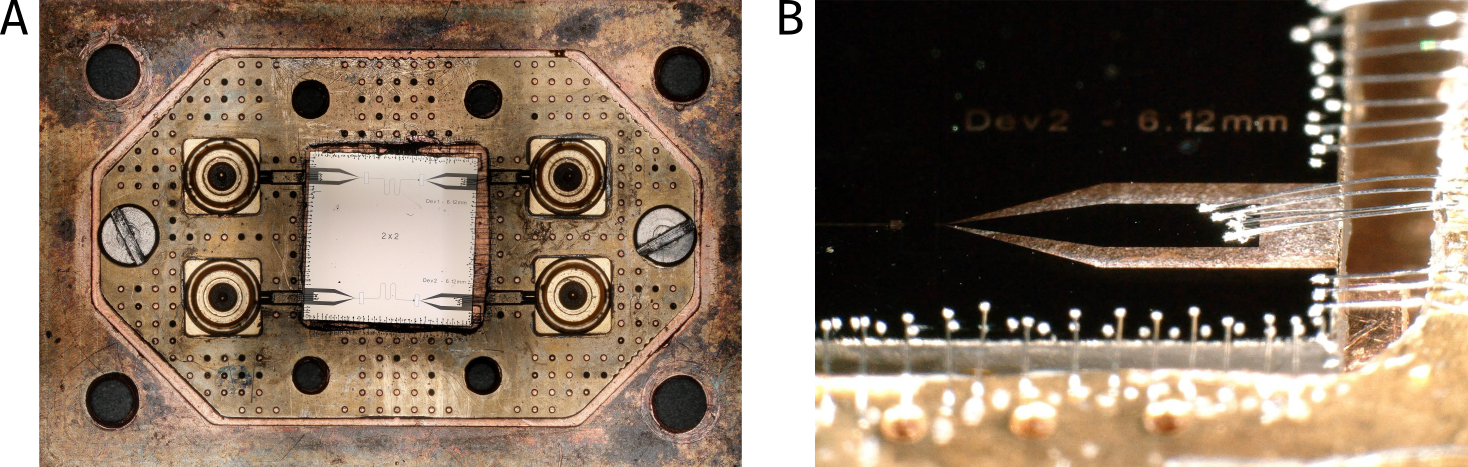
\includegraphics{{chapter-experimental-methods/figs-packaging/packaging.svg}.png}
	\caption{
		\textbf{Device packaging for electrical measurements.}
		% 
		\textbf{A,} A \SI{10x10}{\milli\meter} mounted and wirebonded to a PCB, that is screwed onto a copper base.
		% 
		The four small holes around the chip are used to screw on a small copper lid, covering the chip.
		% 
		The four big holes at the edge of the copper based are used for mounting the chip in a cryostat, and to hold the top cover in place.
		% 
		Connectors for connecting the PCB to the outside world are surface mount SMP plugs.
		% 
		\textbf{B,} Close-up of the bottom-right chip area, taken with ring illumination.
		% 
		The substrate is sapphire, hence the chip transparency.
		% 
		In the bottom right corner, one of the copper rails on which the chip sits is visible.
	}
	\label{fig:packaging}
\end{figure}

